% $Id$
% Author:	Daniel Bosk
\documentclass[a4paper]{article}
\usepackage[utf8]{inputenc}
\usepackage[T1]{fontenc}
\usepackage{xparse}
\usepackage[ibycus,english,swedish]{babel}
\usepackage[strict]{csquotes}
\usepackage[hyphens]{url}
\usepackage{graphicx}
\usepackage[small,bf]{caption}
\usepackage{verbatim}
\usepackage{booktabs}
\usepackage[multiple]{footmisc}
\usepackage[natbib,style=alphabetic,maxbibnames=99]{biblatex}
\addbibresource{introkrypt.bib}

\author{Daniel Bosk\thanks{%
	Detta verk är tillgängliggjort under licensen Creative Commons 
	Erkännande-DelaLika 2.5 Sverige (CC BY-SA 2.5 SE).
	För att se en sammanfattning och kopia av licenstexten besök URL 
	\url{http://creativecommons.org/licenses/by-sa/2.5/se/}.
}}
\title{En introduktion till kryptografi\thanks{%
  Kompendiet är skrivet för att kunna tillgodogöra sig utan förkunskaper andra 
  än nioårig svensk grundskola.
  För avsnitten som behandlar kryptosystemen formellt kan dock mer matematisk 
  vana vara fördelaktig, exempelvis en inledande kurs i diskret matematik på 
  universitetsnivå.
  Men med detta är inte sagt att detta är ett krav, det är fullt möjligt att 
  dessa avsnitt är givande för läsaren ändå.
}}
\date{\today}

\usepackage{amssymb}
\usepackage{amsmath}
\usepackage{amsthm}
\newtheorem{theorem}{Sats}%[chapter]
\newtheorem{lemma}{Lemma}
\newtheorem{corollary}{Korollarium}
\theoremstyle{definition}
\newtheorem{definition}{Definition}
\newtheorem{axiom}[definition]{Axiom}
\newtheorem{example}{Exempel}
\newtheorem{exercise}{Övning}
\theoremstyle{remark}
\newtheorem{remark}{Anmärkning}

\usepackage{varioref}
\renewcommand{\reftextbefore}{(föregående sida)}
\renewcommand{\reftextfacebefore}{(föregående sida)}
\renewcommand{\reftextafter}{(nästa sida)}
\renewcommand{\reftextfaceafter}{(nästa sida)}
\renewcommand{\reftextfaraway}[1]{(sidan~\pageref{#1})}
\usepackage{hyperref}
\usepackage[noabbrev,swedish]{cleveref}
\crefname{conjecture}{förmodan}{förmodan}
\crefname{axiom}{axiom}{axiom}
\crefname{exercise}{övning}{övning}
\Crefname{exercise}{Övning}{Övning}
\crefname{corollary}{korollarium}{korollarium}
%\crefname{proposition}{proposition}{proposition}

\renewcommand{\qedsymbol}{Q.E.D.}

\DeclareDocumentCommand{\N}{}{\ensuremath{\mathbb{N}}}
\DeclareDocumentCommand{\Z}{}{\ensuremath{\mathbb{Z}}}
\DeclareDocumentCommand{\Q}{}{\ensuremath{\mathbb{Q}}}
\DeclareDocumentCommand{\R}{}{\ensuremath{\mathbb{R}}}
\DeclareDocumentCommand{\powerset}{}{\ensuremath{\mathcal{P}}}
\DeclareDocumentCommand{\U}{}{\ensuremath{\mathcal{U}}}
\DeclareDocumentCommand{\V}{}{\ensuremath{\mathcal{V}}}
\DeclareMathOperator{\card}{card}
\DeclareMathOperator{\tnot}{icke}
\DeclareMathOperator{\tor}{eller}
\DeclareMathOperator{\tand}{och}
\DeclareMathOperator{\lequiv}{\Longleftrightarrow}
\DeclareMathOperator{\congruent}{\equiv}

\DeclareMathOperator{\p}{\mathcal{P}}
\let\P\p
\DeclareMathOperator{\C}{\mathcal{C}}
\DeclareMathOperator{\K}{\mathcal{K}}
\DeclareMathOperator{\E}{\mathcal{E}}
\DeclareMathOperator{\D}{\mathcal{D}}

\let\stoch\relax

\renewcommand{\p}{\stoch{P}}
\renewcommand{\c}{\stoch{C}}
\renewcommand{\k}{\stoch{K}}
\newcommand{\x}{\stoch{X}}
\newcommand{\y}{\stoch{Y}}
\newcommand{\e}{\stoch{E}}
\newcommand{\s}{\stoch{S}}

\DeclareMathOperator{\xor}{\oplus}

\begin{document}
\maketitle
\tableofcontents
\clearpage

\section{Inledning}
\label{sec:Inledning}
Ordet kryptografi kommer från grekiskans \ibygr{krupto's} (\emph{kryptos}) och 
\ibygr{gra'fos} (\emph{graphos})~\cite{OED2013cg}.
Dessa betyder \emph{gömd} eller \emph{hemlig}~\cite{OED2013c} respektive 
\emph{skrift}~\cite{OED2013g}.
Ordet kryptografi betyder följaktligen \emph{hemlig skrift}.

Människan har troligtvis använt sig av kryptografi lika länge som skriftspråket 
har funnits, för om vi ser till människans historia har det mer eller mindre 
alltid funnits hemligheter.
Kryptografin har då kunnat utvecklats under väldigt lång tid.
Genom tiderna har det utvecklats många kryptoapparater, vi ska i denna text 
bland annat titta på en av de äldsta.


\section{Terminologi för kryptosystem}
\noindent
När vi pratar om kryptografi används viss terminologi.
Vi har en klartext och ett klartextalfabet.
\emph{Klartexten}\footnote{%
	Engelskans \emph{plaintext}.
}\index{klartext} är det hemliga meddelande som vi vill skydda med hjälp av 
kryptografi.
\emph{Klartextalfabetet}\footnote{%
	Engelskans \emph{plaintext alphabet}.
}\index{klartextalfabet} är det alfabet som används för att skriva klartexten.

Sedan har vi också en kryptotext och ett kryptoalfabet.
\emph{Kryptotext}\footnote{%
	Engelskans \emph{ciphertext}.
}\index{kryptotext} är den resulterande texten som vi får efter att vi 
krypterat vår klartext.
\emph{Kryptoalfabetet}\footnote{%
	Engelskans \emph{ciphertext alphabet}.
}\index{kryptoalfabet} är det alfabet som används för kryptotexten.

I de kryptosystem som finns i denna text används olika delar av det vanliga 
alfabetet som klartextalfabet respektive kryptoalfabet.
För att kunna skilja på vilket som är vilket väljer vi våra gemener för 
klartextalfabetet, exempelvis \emph{abc\dots}, och våra versaler för 
kryptoalfabetet, exempelvis \emph{ABC\dots}.

För att kunna kryptera och avkryptera krävs en \emph{hemlig nyckel}\footnote{%
	Engelskans \emph{secret key}.
}\index{hemlig nyckel}, det är alltså nyckeln som ska hållas hemlig.
För att kunna avkryptera ett hemligt meddelande, en kryptotext, krävs nyckeln.
Med fel nyckel ger avkrypteringen bara en text med osammanhängande 
kombinationer av tecken från klartextalfabetet.

\subsection{Formell definition av ett kryptosystem}
\noindent
Låt oss inleda med att definiera vad vi menar när vi skriver kryptosystem.
Vi kommer i denna text att använda samma matematiska notation som 
\citet{Stinson2006cta}.
\begin{definition}\label{def:kryptosystem}
  Ett \emph{kryptosystem}\index{kryptosystem!formell definition} är en tupel 
  \((\P, \C, \K, \E, \D)\) där följande gäller:
  \begin{enumerate}
    \item \(\P\) är en ändlig mängd av möjliga klartexter.
    \item \(\C\) är en ändlig mängd av möjliga kryptotexter.
    \item \(\K\), kallad \emph{nyckelrymden}, är en ändlig mängd av möjliga 
      nycklar.
    \item För varje \(k\in \K\) finns en 
      \emph{krypteringsregel}\index{krypteringsregel} \(e_k\in \E\) och 
      motsvarande \emph{avkrypteringsregel}\index{avkrypteringsregel} \(d_k\in 
      \D\).
      Varje \(e_k\colon \P\to \C\) och \(d_k\colon \C\to \P\) är funktioner 
      sådana att \(d_k(e_k(p)) = p\) för alla klartexter \(p\in \P\).
  \end{enumerate}
\end{definition}
Det är den sistnämda egenskapen som gör att vi kan kommunicera utan 
tvetydigheter.
Samma egenskap säger också att det är nyckeln \(k\) som måste hållas hemlig för 
att vår kommunikation ska hållas säker.

\section{Permutationschiffer}
\label{sec:permutations}
En av de tidigare uppfinningarna som kunnat tillämpas inom kryptografin var ett 
redskap som heter \emph{skytale}\index{skytale}.
Den bestod av en pinne av en given tjocklek och en läderrem.
Läderremmen lindades runt pinnen, och därefter skrevs det hemliga meddelandet 
på remmen.
Se bild i \cref{fig:Skytale}.
När meddelandet var klart lindades läderremmen av från pinnen och den fördes 
till mottagaren.
För att kunna läsa texten på läderremmen krävdes att läsaren lindade upp remmen 
på en pinne av samma tjocklek som användes vid skapandet av meddelandet.
Om en pinne av fel diameter används kommer bokstäverna att hamna fel och texten 
blir oläsbar.
\begin{figure*}
	\centering
  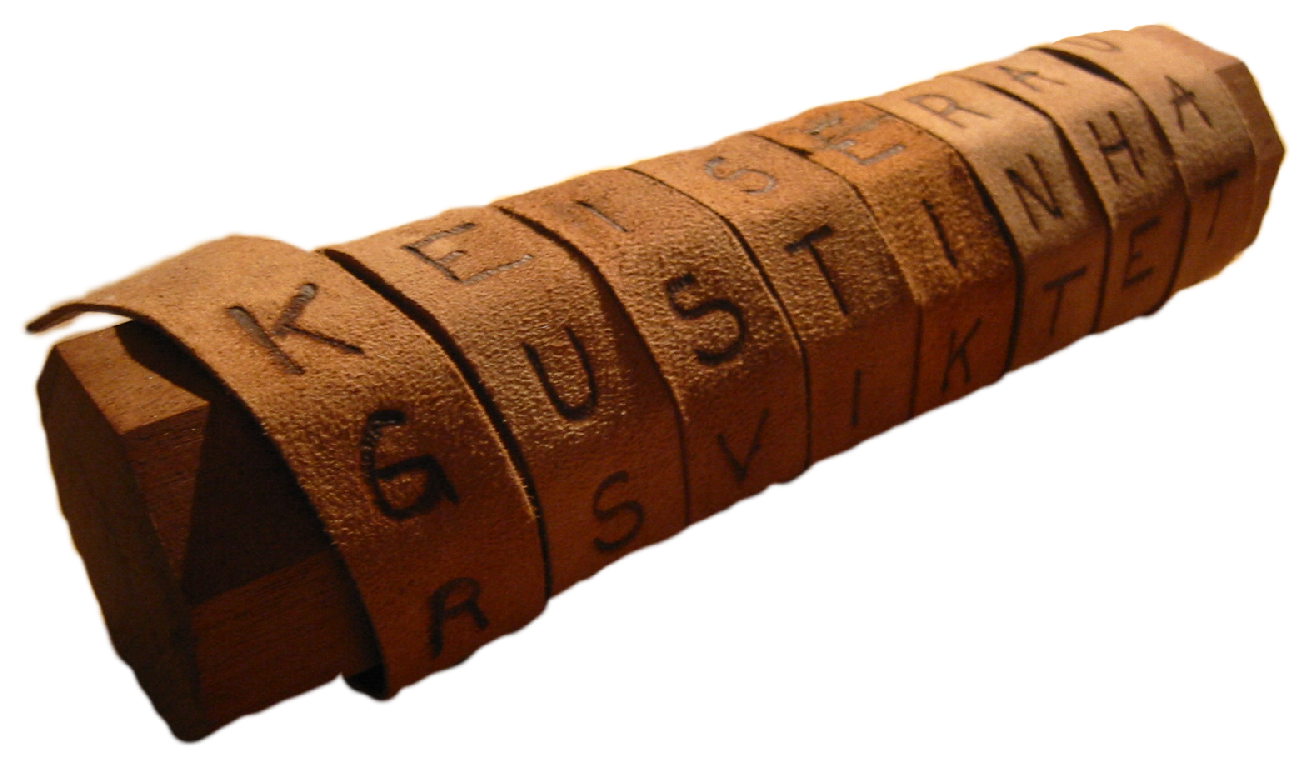
\includegraphics[width=7cm]{figs/skytale.eps}
  \caption{%
    En skytale där texten ''\textsc{keiser augustin \dots}''
		skrivits.
    Bild:~\cite{Wikipedia2011s}.
  }\label{fig:Skytale}
\end{figure*}

Det är dock omdebatterat huruvida denna \enquote{kryptoapparat} uppfanns med 
syfte att vara en kryptoapparat eller bara en metod att lagra meddelanden eller 
en metod att verifiera avsändare~\cite{Kelly1998tmo}.
Hur det än är kan den tillämpas på sådant sätt att det blir ett chiffer, och 
det chiffret tittar vi på här.

Det chiffer som används i kryptoapparaten skytale kan generaliseras enligt 
följande.
Först bestäms bredd och höjd för en rektangel av rutor, där en bokstav ska 
skrivas i varje ruta.
Därefter skrivs texten radvis i rutorna i rektangeln.
Då kan den krypterade texten läsas kolumnvis istället för radvis.
\begin{example}\label{ex:skytaleEnDagIJuni}
	Vi vill kryptera texten \emph{En dag i juni}.
	Vi använder radbredden 7 och kolumnhöjden 2 och markerar tomma rutor med en 
	punkt.
	Vi får då
	\begin{verbatim}
    en_dag_
    i_juni.
  \end{verbatim}
  Kryptotexten blir då \emph{EIN\_\_JDUANGI\_.}.
  För att avkryptera skriver vi bara texten i samma rektangel.
  \begin{verbatim}
    EN_DAG_
    I_JUNI.
  \end{verbatim}
\end{example}
Om vi vill skriva ett längre meddelande används flera rutor.

Denna typ av chiffer kallas för 
\emph{transpositions-}\index{transpositionschiffer} eller 
\emph{permutationschiffer}\footnote{%
	Engelskans \emph{transposition cipher} eller \emph{permutation cipher}.
}\index{permutationschiffer}.

\subsection{Formell definition av permutationschiffer}
Formellt definierar vi ett permutationschiffer enligt följande.
\begin{definition}[Permutationschiffer]\label{def:permutationCipher}\index{permutationschiffer!formell 
    definition}
  Låt \(n\) vara ett positivt heltal och \(A\) ett alfabet.
  Låt också \(\P = \C = A^n\) och låt \(\K\) vara alla möjliga permutationer av 
  mängden \(\{1,\ldots,n\}\).
  För en permutation \(\pi\in \K\) definierar vi
  \begin{align}
    \nonumber
    e_\pi(p_1,\ldots,p_n) = (p_{\pi(1)},\ldots,p_{\pi(n)}),
  \end{align}
  för alla klartexter \(p = (p_1,\ldots,p_n)\in \P\), och
  \begin{align}
    \nonumber
    d_\pi(c_1,\ldots,c_n) = (c_{\pi^{-1}(1)},\ldots,c_{\pi^{-1}(n)}),
  \end{align}
  för alla kryptotexter \(c = (c_1,\ldots,c_n)\in \C\) och där \(\pi^{-1}\) är 
  den inverterade permutationen \(\pi\).
\end{definition}

Låt oss illustrera definitionen genom att tillämpa den på 
\cref{ex:skytaleEnDagIJuni}.
\begin{example}\label{ex:permutationEnDagIJuni}
  Låt \(n = 7\times 2 = 14\).
  Vi låter också permutationen \(\pi\in \K\) definieras enligt 
  \cref{tbl:pi}.
  \begin{table*}
    \caption{%
      Definitionen av permutationen \(\pi\).
    }\label{tbl:pi}
    \centering
    \begin{tabular}{rrrrrrrrrrrrrrr}
      \toprule
      \(i\)       & 1 & 2 & 3 & 4 & 5 & 6 & 7 & 8 & 9 & 10 & 11 & 12 & 13 & 14 
      \\
      \(\pi(i)\)  & 1 & 8 & 2 & 9 & 3 & 10 & 4 & 11 & 5 & 12 & 6 & 13 & 7 & 14 
      \\
      \bottomrule
    \end{tabular}
  \end{table*}
  För att kryptera använder vi \(e_\pi\in \E\).
  Om vi låter \(p = (p_1, \ldots, p_n)\) vara vår klartext \enquote{en dag 
    i juni}, alltså \(p_1 = e, p_2 = n\) och så vidare, får vi att \(c 
    = e_\pi(p) = (p_1, p_8, p_2, p_9, \ldots, p_7, p_{14})\) och således att 
  \(c\) är vår kryptotext \enquote{EIN\_\_JDUANGI\_.}.

  Vi avkrypterar på samma sätt med hjälp av \(\pi^{-1}\).
\end{example}

Om vi vill kryptera ett meddelande som är längre upprepas användningen av 
permutationen, exempelvis om permutationen i \cref{tbl:pi} används 
krypteras 14 tecken åt gången.
Notera dock att en klartext som ska krypteras med denna metod måste vara jämnt 
delbar med storleken för permutationen: 14, 28, \dots, i fallet ovan.
Om detta inte är fallet kan någon form av fyllnadstecken läggas till för att få 
rätt blockstorlek.

Vi ser också ganska omedelbart att antalet möjliga nycklar \(|\K| = {n!}\) 
växer snabbt med antalet bokstäver \(n\) i ett block som permuteras.

\begin{exercise}
  Skapa en permutation av längden \(n = 5\).
  Använd denna för att kryptera en klartext som är minst tio tecken lång.
\end{exercise}
\begin{exercise}
  Byt den resulterande kryptotexten från föregående uppgift med någon annan.
  Börja med att försöka lista ut permutationen som använts vid skapandet av 
  kryptotexten du fått.
  Använd därefter rätt permutation och avkryptera meddelandet.
  Verifiera att du kommit fram till rätt klartext.
\end{exercise}
\begin{exercise}
  Undersök vad som händer vid sammansättning av permutationer.
  Exempelvis om permutationen \(\pi\) i \cref{tbl:pi} appliceras två 
  gånger, eller att två olika permutationer kombineras: spelar det då någon 
  roll i vilken ordning de appliceras?
\end{exercise}

För vidare studier av permutationer, se avsnitt 10.6 och kapitel 21 i Biggs bok 
\emph{Discrete Mathematics}~\cite{Biggs2002dm}.

\begin{exercise}
  Försök att finna en kryptotext \(c\) och två nycklar, \(k\) och \(k^\prime\), 
  sådana att \(d_k(c)\) och \(d_{k^\prime}(c)\) ger tolkningsbara klartexter då 
  permutationschiffret används som kryptosystem.
\end{exercise}
\begin{exercise}
  Varför är det intressant att finna kryptotexter som beroende av nyckel kan 
  avkrypteras till olika läsbara klartexter?
\end{exercise}


\section{Caesarchiffer}
\label{sec:Caesar}
\index{Caesarchiffer}
Chiffret vi ska titta på i detta avsnitt är uppkallat efter den romerske 
diktatorn och kejsaren Julius Caesar (49 f.Kr. -- 44 e.Kr.).
Även om chiffret troligtvis uppfunnits tidigare har det fått detta namn 
eftersom att Caesar lär ha använt det med nyckeln given 
i \cref{tbl:Caesarchiffer}~\cite{Stinson2006cta}.
Chiffret är annars även känt som ett skiftchiffer, vi kommer att se varför.

Chiffret använder det vanliga alfabetet som både klartext- och kryptoalfabete.
För att kryptera förskjuts kryptoalfabetet mot klartextalfabetet ett givet 
antal steg.
Det är antalet steg som utgör nyckeln i Caesarchiffret.
Därefter krypteras meddelandet genom att varje klartextbokstav motsvaras av en 
kryptotextbokstav.
Se \cref{tbl:Caesarchiffer}.

\begin{table*}
  \caption{%
    Tabell för att kryptera med ett Caesarchiffer med nyckeln C.
  }\label{tbl:Caesarchiffer}
	\centering
  \begin{tabular}{ccccccccccccccc}
    \toprule
    a & b & c & d & e & f & g & h & i & j & k & l & m & n & o \\
		C & D & E & F & G & H & I & J & K & L & M & N & O & P & Q \\
    \midrule
    p & q & r & s & t & u & v & w & x & y & z & å & ä & ö \\
		R & S & T & U & V & W & X & Y & Z & Å & Ä & Ö & A & B \\
    \bottomrule
  \end{tabular}
\end{table*}

\begin{example}
  För att kryptera klartexten \emph{hej} slår man upp bokstav för bokstav 
  i \cref{tbl:Caesarchiffer}.
	Det vill säga, \emph{h $\mapsto$ J}, \emph{e $\mapsto$ G} och 
	\emph{j $\mapsto$ L}.
	Kryptotexten blir alltså \emph{JGL}.
\end{example}

\begin{example}\label{ex:CaesarSkatten}
	Om vi krypterar ordet \emph{skatten} blir det \emph{UMCVVGP}.
\end{example}

\subsection{Formell definition av Caesarchiffret}
Låt oss ge följande definition av Caesar- eller skiftchiffret.
\begin{definition}[Skiftchiffer]\label{def:shiftCipher}\index{Caesarchiffer!formell 
    definition}\index{skiftchiffer!formell definition}
  Låt \(\P = \C = \K = \Z_{29}\) och låt varje bokstav i det svenska alfabetet 
  motsvara ett unikt tal i \(\Z_{29}\).
  För alla \(k\in \K\) definierar vi
  \begin{align}
    \nonumber
    e_k(p) &= (p + k) \bmod 29, \text{\ och\ } \\
    \nonumber
    d_k(c) &= (c - k) \bmod 29,
  \end{align}
  där \(p\in \P\) är en klartextbokstav och \(c = e_k(p)\in \C\) är motsvarande 
  kryptotextbokstav.
\end{definition}

Vi förtydligar definitionen med ett exempel.
\begin{example}\label{ex:shiftdef}
  Låt oss numrera bokstäverna i det svenska alfabetet enligt index med start 
  från noll.
  Då får vi att textsträngen \enquote{hej} skulle kunna motsvaras av tupeln \(p 
    = (7, 4, 9)\).
  Om vi låter nyckeln \(k\in \K\) vara \(2\) får vi att
  \begin{align}
    \nonumber
    c = e_2(p) &= (e_2(7), e_2(4), e_2(9)) \\
    \nonumber
      &= (9, 6, 11).
  \end{align}
  Om vi översätter tillbaka till bokstäver får vi att \(c\) motsvarar strängen 
  \enquote{JGL}.
\end{example}

Vi ser här att antalet möjliga nycklar \(|\K| = |\Z_{29}| = 29\) är alldeles 
för få.

\begin{exercise}
  Försök att finna en kryptotext \(c\) och två nycklar, \(k\) och \(k^\prime\), 
  sådana att \(d_k(c)\) och \(d_{k^\prime}(c)\) ger tolkningsbara klartexter då 
  Caesarchiffret används som kryptosystem.
\end{exercise}
\begin{exercise}
  Hur påverkar längden av kryptotexten i förhållandet till kryptosystemets 
  blockstorlek, i Caesarchiffrets fall är blockstorleken en bokstav?
\end{exercise}

\subsection{Kryptanalys av Caesarchiffret}
\label{sec:KryptanalysCaesar}
\index{Caesarchiffer!kryptanalys}
Caesarchiffret är inte ett särskilt säkert sätt att skydda information.
Det är lätt att knäcka.
Det finns totalt, om det svenska alfabetet används, 29 olika nycklar som kan 
användas för kryptering och avkryptering eftersom att alfabetet maximalt kan 
förskjutas lika många steg som det finns bokstäver\footnote{%
	Detta kan beräknas genom att vi på den första platsen kan välja mellan 29 
	bokstäver, på de efterföljande platserna kan då bara välja en bokstav.  Vi 
	får då totala antalet nycklar genom \(29\cdot 1\cdot 1\cdots 1 = 29\).
}.
Detta är så få att det till och med enkelt kan testas för hand för att lista ut 
vilken nyckel som använts.
Om det finns tillgång till en dator och man kan programmera, då är det ännu 
enklare.
Men det går tack vare språkets egenskaper att reducera antalet nycklar som 
behöver testas ytterligare.
Titta på \cref{ex:CaesarSkatten} där \emph{tt} blir \emph{VV}, det är 
långt från alla bokstäver i svenskan som upprepas på detta sätt.
I \cref{sec:KryptanalysSubstitution} ska vi se ytterligare ett sätt att 
kryptanalysera Caesarchiffret på.

\begin{exercise}\label{xrc:caesarAddition}
  Låt \(c\) och \(c^\prime\) vara två kryptotexter krypterade med samma nyckel 
  \(k\).
  Det vill säga \(c = e_k(m) = (m_1+k, m_2+k, \ldots, m_n+k)\) och \(c^\prime 
  = e_k(m^\prime) = (m^\prime_1+k, m^\prime_2+k, \ldots, m^\prime_n+k)\), där 
  alla aritmetiska operationer görs modulo 29.
  Undersök vad som händer då vi utför aritmetik med \(c\) och \(c^\prime\), 
  exempelvis \(c - c^\prime \mod 29\).
  Hur påverkar detta inflytandet av nyckeln \(k\) på kryptotexten?
\end{exercise}


\section{Substitutionschiffer}
\label{sec:Substitution}
I ett \emph{substitutionschiffer}\index{substitutionschiffer} avbildas varje 
bokstav i klartextalfabetet på en unik bokstav i kryptoalfabetet.
Caesarchiffret är alltså ett substitutionschiffer.
I dagstidningar, bland korsorden, brukar det finnas en typ av korsord som 
kallas för krypto, där rutorna är markerade med tal och varje tal motsvarar en 
bokstav.
Här används alltså det vanliga alfabetet, \(a, b, c, \cdots\), som 
klartextalfabete och talen \(1,2,3,\ldots, 29\) som kryptoalfabete.
Nyckeln i substitutionschiffret utgör hela avbildningen mellan klartext- och 
kryptoalfabetet.
Ett exempel visas i \cref{tbl:Substitutionschiffer}.

\begin{table*}
  \caption{%
    Tabell för att kryptera med ett substitutionschiffer.
		Gemener används som klartextalfabete och versaler som kryptoalfabete.
  }\label{tbl:Substitutionschiffer}
	\centering
	\begin{tabular}{ccccccccccccccc}
    \toprule
    a & b & c & d & e & f & g & h & i & j & k & l & m & n & o \\
		C & M & Q & F & Z & Ö & I & J & P & L & D & N & O & K & D \\
    \midrule
    p & q & r & s & t & u & v & w & x & y & z & å & ä & ö \\
		R & S & T & Å & V & Y & X & W & G & U & Ä & H & A & B \\
    \bottomrule
  \end{tabular}
\end{table*}

För att kryptera gör man på samma sätt som i Caesarchiffret.

\begin{example}\label{ex:SubstitutionHej}
  För att kryptera klartexten \emph{hej} slår man upp bokstav för bokstav 
  i \cref{tbl:Substitutionschiffer}.
	Det vill säga, \(h\mapsto J\), \(e\mapsto Z\) och 
	\(j\mapsto L\).
	Kryptotexten blir alltså \emph{JZL}.
\end{example}

\begin{example}\label{ex:SubstitutionSkatten}
	Om vi krypterar ordet \emph{skatten} blir det \emph{ÅDCVVZK}.
\end{example}

\subsection{Formell definition av substitutionsciffer}
Vi definierar substitutionschiffret som följer.
För enkelthet använder vi samma alfabet för både klartext och kryptotext, även 
om detta inte är en nödvändig begränsning.
Om vi vill ha ett annat kryptoalfabet är detta egentligen bara en fråga om 
kodning, och detta kan läggas till i efterhand.
\begin{definition}[Substitutionschiffer]\label{def:substitutionCipher}\index{substitutionschiffer!formell 
    definition}
  Låt \(A\) vara vårt alfabet och låt \(\P = \C = A\).
  Vidare låt \(\K\) bestå av alla möjliga permutationer av \(A\).
  För varje permutation \(\pi\in \K\) definierar vi att
  \begin{align}
    \nonumber
    e_\pi(p) &= \pi(p), \text{\ och\ } \\
    \nonumber
    d_\pi(c) &= \pi^{-1}(c),
  \end{align}
  där \(\pi^{-1}\) är den inverterade permutationen \(\pi\), \(p\in \P\) är en 
  klartextbokstav och \(c = e_\pi(p)\in \C\) är motsvarande kryptotextbokstav.
\end{definition}

Notera skillnaden mellan användningen av permutationen \(\pi\) i denna 
definition och den i \cref{def:permutationCipher}.
I den tidigare användes permutationen på index i ett block medan i denna 
definition används permutationen direkt på enskilda tecken.
Här permuteras bokstaven medan i den tidigare permuterades bokstavens position.

Vi förtydligar definitionen med följande exempel.
\begin{example}
  Vi kan här återanvända \cref{ex:SubstitutionHej}.
  Vi låter \(A\) vara det svenska alfabetet.
  Nyckeln \(\pi\in \K\) kan vi låta vara densamma som 
  i \cref{ex:SubstitutionHej}, vilken vi ser 
  i \cref{tbl:Substitutionschiffer}.
  Då får vi att \(e_\pi(h) = J, e_\pi(e) = Z, e_\pi(j) = L\).
\end{example}

Värt att notera är att antalet möjliga nycklar \(|\K| = {|A|!}\) växer snabbt 
med storleken av alfabetet.

\begin{exercise}
  Undersök vad som händer vid sammansättning av permutationer i detta chiffer.
  Exempelvis om permutationen \(\pi\) i \cref{def:substitutionCipher} 
  appliceras två gånger, eller att två olika permutationer kombineras: spelar 
  det då någon roll i vilken ordning de appliceras?
\end{exercise}
\begin{exercise}
  Försök att finna en kryptotext \(c\) och två nycklar, \(k\) och \(k^\prime\), 
  sådana att \(d_k(c)\) och \(d_{k^\prime}(c)\) ger tolkningsbara klartexter då 
  med detta kryptosystem.
\end{exercise}

\subsection{Kryptanalys av substitutionschiffer}
\label{sec:KryptanalysSubstitution}
\index{substitutionschiffer!kryptanalys}
För generella substitutionschiffer finns det väsentligen fler möjliga nycklar 
än de 29 möjligheter som fanns för Caesarchiffret, men till kostnad av en 
längre nyckel som är svårare att memorera.
Som första bokstav i nyckeln kan vi välja mellan alla 29 bokstäverna i 
alfabetet.
För varje bokstav vi kan välja som första bokstav finns det 28 bokstäver kvar 
som då kan välja mellan.
Vi får således \[29! = 29\cdot 28\cdot 27\cdots 3\cdot 2\cdot 1 =
8841761993739701954543616000000\] möjliga nycklar\footnote{%
  \({29!}\) uttalas \emph{29 fakultet}.
}, vilket gör det svårt att testa alla möjliga nycklar som vi kunde göra med 
Caesarchiffret.
Vi behöver alltså en annan metod.

Vi analyserar följande text: \enquote{An English text has no Swedish letters}.
Vi vill nu beräkna sannolikheten att välja en specifik bokstav om vi väljer en 
slumpmässig bokstav i denna mening.
Det vill säga, vi väljer en slumpmässig bokstav från mängden
\begin{align}
  \nonumber
  A = \{a, n, e, g, l, i, s, h, t, x, o, w, d, r\}.
\end{align}
Låt \(\x\) beteckna en stockastisk variabel som antar värden ur \(A\).
Vi vet från sannolikhetsläran att sannolikheten \(\Pr(\x = a)\) att vi väljer 
\emph{a} och att detta värde beräknas som
\begin{equation}
  \nonumber
  \Pr(\x = \alpha) = \frac{\#\alpha}{N},
\end{equation}
där \(\#\alpha\) är antalet förkomster av \(\alpha\) i texten och \(N\) är 
totala antalet tecken i texten.
Vi kan då beräkna att \(\Pr(\x = a) = 0.0625\) och alltså att sannolikheten att 
en slumpvis vald bokstav i texten är ett \emph{a} är 6.25 procent.
Värdena av \(\Pr(\x = \alpha)\) för samtliga värden av \(\alpha\) ges 
i \cref{tbl:SannolikhetstabellKlartext}.

\begin{table*}
  \caption{%
    Tabell av sannolikhetsfördelningen för den stokastiska variabeln \(\x\) som 
    antar bokstäver i meningen \enquote{anenglishtexthasnoswedishletters}, 
    angiven med tre decimalers noggrannhet.
  }\label{tbl:SannolikhetstabellKlartext}
	\centering
  \begin{tabular}{rcccccccccc}
    \toprule
    \(\alpha\) & a & b & c & d & e & f & g & h & i & j  \\
    \(\Pr(\x = \alpha)\) & 0.063  & 0.000 & 0.000 & 0.031 & 0.156 & 0.000 
    & 0.031 & 0.094 & 0.064 & 0.000 \\
    \midrule
    \(\alpha\) & k & l & m & n & o & p & q & r & s & t \\
    \(\Pr(\x = \alpha)\) & 0.000 & 0.063 & 0.000 & 0.094 & 0.031 & 0.000 
    & 0.000 & 0.031 & 0.156 & 0.125 \\
    \midrule
    \(\alpha\) & u & v & w & x & y & z & å & ä & ö \\
    \(\Pr(\x = \alpha)\) & 0.000 & 0.000 & 0.031 & 0.031 & 0.000 & 0.000 
    & 0.000 & 0.000 & 0.000 \\
    \bottomrule
  \end{tabular}
\end{table*}
\begin{table*}
  \caption{%
    Tabell av sannolikhetsfördelningen för den stokastiska variabeln \(\y\) som 
    antar bokstäver i meningen \enquote{CPGPINKUJVGZVJCUPQUYGFKUJNGVVGTU}, 
    angiven med tre decimalers noggrannhet.
  }\label{tbl:SannolikhetstabellKryptotext}
	\centering
  \begin{tabular}{rcccccccccccc}
    \toprule
    \(\alpha\) & A & B & C & D & E & F & G & H & I & J \\
    \(\Pr(\y = \alpha)\) & 0.000 & 0.000 & 0.063  & 0.000 & 0.000 & 0.031 
    & 0.156 & 0.000 & 0.031 & 0.094 \\
    \midrule
    \(\alpha\) & K & L & M & N & O & P & Q & R & S & T \\
    \(\Pr(\y = \alpha)\) & 0.064 & 0.000 & 0.000 & 0.063 & 0.000 & 0.094 
    & 0.031 & 0.000 & 0.000 & 0.031 \\
    \midrule
    \(\alpha\) & U & V & W & X & Y & Z & Å & Ä & Ö \\
    \(\Pr(\y = \alpha)\) & 0.156 & 0.125 & 0.000 & 0.000 &  0.031 & 0.031 
    & 0.000 & 0.000 & 0.000 \\
    \bottomrule
  \end{tabular}
\end{table*}

Om vi krypterar en text med ett substitutionschiffer, exempelvis ett 
Caesarchiffer, då förändrar vi inte antalet av någon bokstav, det enda vi 
ändrar är bokstavens representation (''utseende'').
Vi krypterar \enquote{anenglishtexthasnoswedishletters} med något okänt 
substitutionschiffer och får då
\begin{quote}
  CPGPINKUJVGZVJCUPQUYGFKUJNGVVGTU\@.
\end{quote}
Vi låter den stokastiska variabeln \(\y\) anta bokstäver i meningen ovan.
Sannolikhetsfördelningen för \(\y\) är tabellerad 
i \cref{tbl:SannolikhetstabellKryptotext}.
Om vi tittar i tabellen ser vi att \(\Pr(\x = a) = \Pr(\y = C) = \Pr(\y = N)\), 
då har vi alltså två alternativ som skulle kunna representera \emph{a} 
i kryptoalfabetet.
Ett bra riktmärke kan vara att titta på den vanligaste bokstaven, 
i klartextalfabetet är det \emph{e} med \(\Pr(\x = e) = 0.156\).
Det är då mycket möjligt att \(e\mapsto G\) eftersom att \(\Pr(\y = G)\) också 
är \(0.156\).
Ytterligare information vi kan använda är återupprepningar hos bokstäver,
jämför med \cref{ex:CaesarSkatten} och~\ref{ex:SubstitutionSkatten}
där t:et i ordet \emph{skatten} upprepar sig.
De enda bokstäver som upprepar sig i svenskan är konsonanter, och bokstäverna 
omkring dessa är oftast vokaler.
Av vad vi sett hittills verkar det som att kryptotexten är krypterad med ett 
Caesarchiffer med nyckeln C eftersom att \(a\mapsto C\) och \(e\mapsto G\) är 
troliga avbildningar.
Om vi testar att avkryptera enligt Caesarchiffret med nyckeln C ser vi att vår 
gissning var korrekt.

Nu kände vi till sannolikhetsfunktionen för klartexten när vi tittade på
kryptotexten, men hur gör man egentligen när man inte vet någonting om 
klartexten?
Om man har tillräckligt mycket text kommer sannolikhetsfunktionen för texten att 
närma sig sannolikhetsfunktionen för språket.
Då kan textens sannolikhetsfunktion jämföras för att först se vilket språk 
texten är skriven på och därefter kan man hitta nyckeln som vi gjorde ovan.
Sannolikhetsfunktionen för språken svenska och engelska finns givna i 
\cref{tbl:SannolikhetstabellSpråk}.
En överblicksbild för det engelska språket ges även 
i \cref{fig:SannolikhetstabellEngelska}.
Sannolikhetstabeller för några olika språk finns tillgängliga hos 
\cite{Wikipedia2013lf}.

\begin{table*}
  \caption{%
    Tabell av sannolikhetsfördelningen för bokstäver i det 
    engelska~\cite{Stinson2006cta} och det svenska~\cite{Wikipedia2013lf} 
    språket, den stokastiska variabeln \(\e\) respektive \(\s\), angiven med 
    tre decimalers noggrannhet.
  }\label{tbl:SannolikhetstabellSpråk}
	\centering
  \begin{tabular}{rcccccccccc}
    \toprule
    \(\alpha\) & a & b & c & d & e & f & g & h & i & j \\
    \(\Pr(\e = \alpha)\) & 0.082  & 0.015 & 0.028 & 0.043 & 0.127 & 0.022 
    & 0.020 &
    0.061 & 0.070 & 0.002 \\
    \(\Pr(\s = \alpha)\) & 0.093  & 0.013 & 0.013 & 0.045 & 0.099 & 0.020 
    & 0.033 &
		0.021 & 0.051 & 0.007 \\
    \midrule
    \(\alpha\) & k & l & m & n & o & p & q & r & s & t \\
    \(\Pr(\e = \alpha)\) & 0.008 & 0.040 & 0.024 & 0.067 & 0.075 & 0.019 
    & 0.001 & 0.060 & 0.063 & 0.091 \\
    \(\Pr(\s = \alpha)\) & 0.032 & 0.052 & 0.035 & 0.088 & 0.041 & 0.017 
    & 0.000 & 0.083 & 0.063 & 0.087 \\
    \midrule
    \(\alpha\) & u & v & w & x & y & z & å & ä & ö \\
    \(\Pr(\e = \alpha)\) & 0.028 & 0.010 & 0.023 & 0.001 & 0.020 & 0.001 
    & 0.000 & 0.000 & 0.000 \\
    \(\Pr(\s = \alpha)\) & 0.018 & 0.024 & 0.000 & 0.001 & 0.006 & 0.000 
    & 0.016 & 0.021 & 0.015 \\
    \bottomrule
  \end{tabular}
\end{table*}

\begin{figure*}
	\centering
  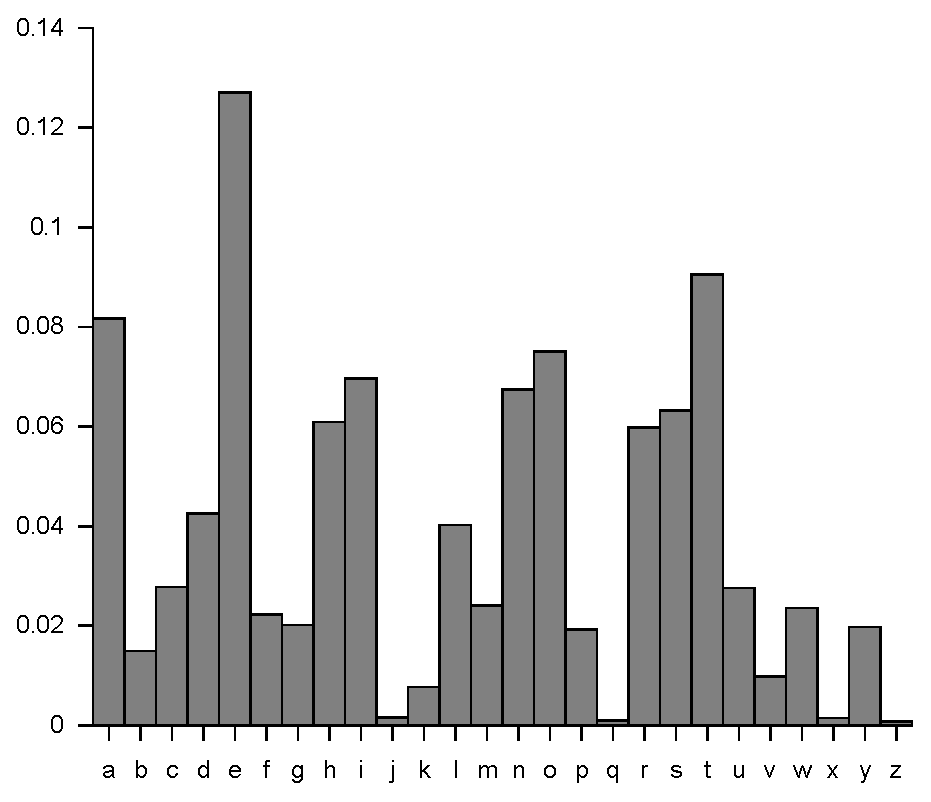
\includegraphics[width=0.7\linewidth]{figs/english_letter_frequencies.eps}
  \caption{%
    En överblickande graf över sannolikhetsfördelningen för den stokastiska 
    variabeln \(\e\).
    Bild:~\cite{Wikipedia2013lf}.
  }\label{fig:SannolikhetstabellEngelska}
\end{figure*}

\begin{exercise}
  Du jobbar som kryptoanalytiker åt Försvarets Radioanstalt (FRA) och får 
  följande text på ditt skrivbord:
  % XXX rewrite plaintext examples to Swedish
	\begin{verbatim}
    VJGOCFJCVVGTUVGCRCTVUWPFGTYC
    KVKUKPVJGWUWCNRNCEGDGJKPFVJGEWTVCKP
  \end{verbatim}
  \begin{comment}
  \begin{verbatim}
    THN MJNSXNGKD RM PNTTNJW AG TNZT HUW RMTNG CNNG WTXVANV MRJ XWN AG
    KJDQTRIJUQHD, UGV MJNSXNGKD UGUPDWAW AG QUJTAKXPUJ. GR NZUKT PNTTNJ
    MJNSXNGKD VAWTJACXTARG XGVNJPANW U IAYNG PUGIXUIN, WAGKN UPP EJATNJW
    EJATN WPAIHTPD VAMMNJNGTPD. PAGRTDQN FUKHAGNW WRJTNV THN PNTTNJW'
    MJNSXNGKANW UW NTURAG WHJVPX KFMEDQ YCIOSL ZB CUWNV RG THN NZQNJANGKN
    UGV KXWTRF RM FUGXUP KRFQRWATRJW. PAONEAWN, FRVNJG AGTNJGUTARGUP FRJWN
    KRVN NGKRVNW THN FRWT MJNSXNGT PNTTNJW EATH THN WHRJTNWT WDFCRPW;
    UJJUGIAGI THN FRJWN UPQHUCNT AGTR IJRXQW RM PNTTNJW THUT JNSXAJN NSXUP
    UFRXGTW RM TAFN TR TJUGWFAT, UGV THNG WRJTAGI THNWN IJRXQW AG
    AGKJNUWAGI RJVNJ, DANPVW N AT WUG HXJVF EIYPMCO RQLZKB DS. WAFAPUJ
    AVNUW UJN XWNV AG FRVNJG VUTU-KRFQJNWWARG TNKHGASXNW WXKH UW HXMMFUG
    KRVAGI.
  \end{verbatim}
	\end{comment}
	Vad betyder det?

	\begin{comment}
		För att knäcka krypteringen gör man en frekvensanalys av bokstäverna.
		Bokstavsfrekvenser för olika språk finns på
		\begin{center}
			\url{http://en.wikipedia.org/wiki/Letter_frequency#Relative_frequencies_of_letters_in_the_English_language}.
		\end{center}

		Det krypterade meddelandet är
		\begin{quote}
      the mad hatter's teaparty is underway\@. it is in the usual place,
			behind the curtain.
		\end{quote}
		\begin{quotation}\noindent
      the frequency of letters in text has often been studied for use in 
      cryptography, and frequency analysis in particular\@. no exact letter 
      frequency distribution underlies a given language, since all writers 
      write slightly differently\@. linotype machines sorted the letters' 
      frequencies as etaoin shrdlu cmfwyp vbgkqj xz based on the experience and 
      custom of manual compositors\@. likewise, modern international morse code 
      encodes the most frequent letters with the shortest symbols; arranging 
      the morse alphabet into groups of letters that require equal amounts of 
      time to transmit, and then sorting these groups in increasing order, 
      yields e it san hurdm wgvlfbk opjxcz yq\@. similar ideas are used in 
      modern data-compression techniques such as huffman coding.
		\end{quotation}
		Det har krypterats med ett substitutionschiffer som har nyckeln
		\begin{verbatim}
      UCKVNMIHALOPFGRQSJWTXYEZDB.
    \end{verbatim}
	\end{comment}
\end{exercise}


\section{Vigenèrechiffer}
\index{Vigenèrechiffer}
\citet{Singh2000tcb} har i sin bok \emph{Kodboken} gjort en kartläggning över 
uppkomsten och förekomster av olika chiffer under historiens gång.
Enligt honom lades grunden för Vigenèrechiffret under 1400-talet av Leon 
Battista Alberti (1404--1472).
Därefter vidareutvecklades hans idéer först av Johannes Trithemius (1462--1516) 
och sedan av Giambattista della Porta (1535--1615).
Anledningen till att metoden kallas Vigenèrechiffer är enligt honom för att den 
är uppkallad efter Blaise de Vigenère (1523--1596) som gjorde det slutgiltiga 
bidraget till utformningen av chiffret.
Vigenèrechiffret användes länge, det användes till och med av sydstaterna under 
det amerikanska inbördeskriget.

Chiffret består av upprepad användning av Caesarchiffret.
Som nyckel används ett ord, för att vara enkelt att komma ihåg, vilket 
bokstavskombination som helst kan användas.
Vid kryptering av en text krypteras första bokstaven i klartexten med ett 
Caesarchiffer där första bokstaven i Vigenèrenyckeln används som nyckel.
Därefter används den andra, den tredje, och så vidare.
När nyckelordets alla bokstäver använts börjar man om.

\begin{example}\label{ex:VigenereSkatten}
  Om vi vill kryptera order \emph{skatten} ska bokstäverna i nyckeln användas 
  enligt
  \begin{verbatim}
    skatten
    ABCABCA
  \end{verbatim}
  och vi får alltså \emph{SLCTUGN} genom att använda de olika Caesarchiffren 
  i \cref{tbl:Vigenerechiffer}.
\end{example}

\begin{table*}
  \caption{%
    Vigenèrechiffer med nyckeln \emph{ABC}.
  }\label{tbl:Vigenerechiffer}
  \centering
  \begin{tabular}{lcccccccccc}
    \toprule
    Klartext & a & b & c & d & e & f & g & h & i & j \\
    A        & A & B & C & D & E & F & G & H & I & J \\
    B        & B & C & D & E & F & G & H & I & J & K \\
    C        & C & D & E & F & G & H & I & J & K & L \\
    \midrule
    Klartext & k & l & m & n & o & p & q & r & s & t \\
    A        & K & L & M & N & O & P & Q & R & S & T \\
    B        & L & M & N & O & P & Q & R & S & T & U \\
    C        & M & N & O & P & Q & R & S & T & U & V \\
    \midrule
    Klartext & u & v & w & x & y & z & å & ä & ö \\
    A        & U & V & W & X & Y & Z & Å & Ä & Ö \\
    B        & V & W & X & Y & Z & Å & Ä & Ö & A \\
    C        & W & X & Y & Z & Å & Ä & Ö & A & B \\
    \bottomrule
  \end{tabular}
\end{table*}

Notera skillnaden mellan kryptotexten av ordet \emph{skatten} i 
\cref{ex:CaesarSkatten}, \cref{ex:SubstitutionSkatten} och 
\cref{ex:VigenereSkatten}.
Upprepningen av t:et försvinner när Vigenerechiffret används.

\subsection{Formell definition av Vigenèrechiffret}
Vi går vidare med en definition av Vigenèrechiffret.
\begin{definition}[Vigenèrechiffer]\index{Vigenèrechiffer!formell definition}
  Låt \(n\) vara ett positivt heltal.
  Definiera att \(\P = \C = \K = (\Z_{29})^n\).
  För alla nycklar \(k = (k_1,\ldots,k_n)\in \K\), klartexter \(p = (p_1, 
  \ldots, p_n)\in \P\) och kryptotexter \(c = (c_1,\ldots,c_n)\in \C\) 
  definierar vi att
  \begin{align}
    \nonumber
    e_k(p) &= (p_1 + k_1, \ldots, p_n + k_n), \text{\ och\ } \\
    \nonumber
    d_k(c) &= (c_1 - k_1, \ldots, c_n - k_n),
  \end{align}
  där alla operationer utförs i \(\Z_{29}\).
\end{definition}

Vi noterar att den enda skillnaden mellan denna definition och 
\cref{def:shiftCipher} är att \(\P, \C, \K\) definieras som 
\((\Z_{29})^n\) istället för \(\Z_{29}\).
Låter vi \(n = 1\) är dessa system identiska.

Om vi använder gruppen \(\Z_2\) istället för \(\Z_{29}\) kommer vi att arbeta 
med bitsträngar av längden \(n\) bitar.
Detta får effekten att \(e_k(p) = p \xor k\) där \(p\) och \(k\) är bitstängar 
av längd \(n\), det vill säga operationen \emph{bitvis exklusivt eller} (XOR).
Detta är en fundamental operation i dagens datorer.

\begin{exercise}
  Försök att finna en kryptotext \(c\) som är lika lång som nyckeln och två 
  nycklar, \(k\) och \(k^\prime\), sådana att \(d_k(c)\) och 
  \(d_{k^\prime}(c)\) ger tolkningsbara klartexter med detta kryptosystem.
\end{exercise}
\begin{exercise}
  Om vi ändrar villkoret i föregående övning, vad händer då kryptotexten 
  istället är längre än nyckeln?
  Och mer intressant, varför blir det så?
\end{exercise}

\subsection{Kryptanalys av Vigenèrechiffret}
\index{Vigenèrechiffer!kryptanalys}
Eftersom att kryptotexten nu är krypterad med flera Caesarnycklar fungerar inte 
längre metoden som vi tog fram i \cref{sec:KryptanalysSubstitution}.
Friedrich Kasiski (1805--1881) publicerade år 1863 tekniken hur man 
fullständigt knäcker chiffret utan några förkunskaper~\cite{Stinson2006cta}.
Tidigare metoder, före Kasiski, krävde att man kände till delar av klartexten,
att man kunde gissa nyckeln eller kände nyckelns längd.

Med mycket kryptotext är det möjligt att finna upprepningar i kryptotexten.
Avståndet mellan upprepningarna måste vara en multipel av nyckelns längd 
eftersom att samma klartext annars skulle krypteras olika på grund av att olika 
delar av nyckeln används.
Det vill säga, nyckelns längd måste vara en gemensam faktor för alla avstånd 
mellan upprepningar.
Om vi tittar på följande exempel.
\begin{example}\label{ex:VigenereMedUpprepning}
  Ett Vigenèrechiffer med nyckeln \emph{ABCD} används för att kryptera texten 
  \emph{cryptoisshortforcryptography}.
  \begin{verbatim}
    Nyckel:     ABCDABCDABCDABCDABCDABCDABCD
    Klartext:   cryptoisshortforcryptography
    Kryptotext: CSASTPKVSIQUTGQUCSASTPIUAQJB
  \end{verbatim}
  Avståndet mellan den upprepade texten \emph{CSASTP} är 16, från första 
  tecken till första tecken.
  De möjliga nyckellängderna är alltså \(16, 8, 4, 2\) eller \(1\).
\end{example}
Genom att finna flera sådana upprepningar är det möjligt att reducera antalet 
möjliga nyckellängder.

När nyckellängden väl är känd, låt oss säga att den är \(n\) tecken, då skrivs 
kryptotexten med \(n\) teckens bredd.
Som vi ser i \cref{ex:VigenereMedUpprepning} hamnar då alla tecken 
krypterade med samma Caesarnyckel ovanför varandra i en kolumn, se 
\cref{ex:VigenereKolumner}.
\begin{example}\label{ex:VigenereKolumner}
  Ett Vigenèrechiffer med nyckeln \emph{ABCD} används för att kryptera texten 
  \emph{cryptoisshortforcryptography}.
  \begin{verbatim}
    Nyckel:     ABCD
    Klartext:   cryp
                tois
                shor
                tfor
                cryp
                togr
                aphy
    Kryptotext: CSAS
                TPKV
                SIQU
                TGQU
                CSAS
                TPIU
                AQJB
  \end{verbatim}
\end{example}
Eftersom att varje kolumn nu är krypterad endast med ett Caesarchiffer kan vi 
enkelt använda kryptanalysmetoderna från \cref{sec:KryptanalysCaesar}
eller \cref{sec:KryptanalysSubstitution} för att lista ut varje 
Caesarnyckel och därmed hela Vigenèrenyckeln.
I \cref{ex:VigenereKolumner} analyserar vi den första kolumnen för att 
komma fram till att den är krypterad med nyckeln \emph{A}, den andra kolumnen 
är krypterad med nyckeln \emph{B}, och så vidare, och slutligen att 
Vigenèrechiffrets nyckel är \emph{ABCD}.

\begin{exercise}
  Undersök resultatet i \cref{xrc:caesarAddition}, hur tillämpbart är 
  detta för Vigenèrechiffret?
\end{exercise}

\section{Engångschiffer och perfekt sekretess}
Vi inleder detta avsnitt med att definiera vad vi menar med perfekt 
sekretess\footnote{%
  Engelskans \emph{perfect secrecy}.
}.
Detta begrepp publicerades första gången av Shannon~\cite{Shannon1949cto} år 
1949.
\begin{definition}\label{def:perfectSecrecy}\index{perfekt sekretess!formell 
    definition}
  Ett kryptosystem \((\P, \C, \K, \E, \D)\) sägs ha \emph{perfekt sekretess} om 
  \(\Pr(\p = p\mid \c = c) = \Pr(\p = p)\) för alla \(p\in \P\) och \(c\in 
  \C\).
  Det vill säga, sannolikheten a posteriori att en klartext är \(p\) om 
  kryptotexten är \(c\) är densamma som sannolikheten a priori att klartexten 
  är \(p\).
\end{definition}

Låt oss fortsätta med att visa några resultat om perfekt sekretess.
Vi inleder med följande lemma som fastställer för en typ av kryptosystem några 
egenskaper som krävs för att detta system ska tillhandahålla perfekt sekretess.
\begin{lemma}\label{lem:perfectSecrecy}
  Låt \((\P,\C,\K,\E,\D)\) vara ett kryptosystem.
  Om \(|\K| = |\C| = |\P|\) och varje nyckel används med sannolikheten 
  \(1/|\K|\) och det för varje klartext \(p\in \P\) och kryptotext \(c\in \C\) 
  finns en unik nyckel \(k\in \K\) sådan att \(e_k(p) = c\), då tillhandahåller 
  kryptosystemet perfekt sekretess.
\end{lemma}
\begin{proof}
  Antag \(|\K| = |\C| = |\P|\).
  Vidare antag \(\Pr(\k = k) = 1/|\K|\) för alla nycklar \(k\in \K\) och att 
  det för alla klartexter \(p\in \P\) och kryptotexter \(c\in \C\) finns en 
  nyckel \(k\in \K\) sådan att \(e_k(p) = c\) och för alla nycklar 
  \(k^\prime\neq k\) gäller att \(e_{k^\prime}(x)\neq c\).

  Låt \(c\in \C\) vara en godtycklig kryptotext.
  Då har vi att
  \begin{align}
    \nonumber
    \Pr(\c = c) = \sum_{k\in \K}\Pr(\k = k)\Pr(\p = d_k(c)).
  \end{align}
  Eftersom att \(\Pr(\k = k) = 1/|\K|\) för alla möjliga \(k\in \K\) och att 
  nyckeln är unik för varje klartext--kryptotextpar har vi
  \begin{align}
    \nonumber
    \Pr(\c = c) &= \sum_{k\in \K}\frac{1}{|\K|}\Pr(\p = d_k(c)) \\
    \nonumber
      &= \frac{1}{|\K|}\sum_{k\in \K} \Pr(\p = d_k(c)).
  \end{align}
  För en fixerad kryptotext \(c\in \C\) är \(d_k(c)\) en permutation av \(\P\).
  Följaktligen får vi
  \begin{align}
    \nonumber
    \Pr(\c = c) &= \frac{1}{|\K|}\sum_{p\in \P} \Pr(\p = p) \\
    \nonumber
      &= \frac{1}{|\K|}\times 1 = \frac{1}{|\K|}.
  \end{align}

  Vidare har vi att \(\Pr(\c = c\mid \p = p) = \Pr(\k = k)\) tack vare att det 
  är en unik nyckel \(k\in \K\) för varje par av klartext \(p\in \P\) och 
  kryptotext \(c\in \C\).

  % XXX cross-reference Bayes' theorem, \cref{thm:Bayes}
  Slutligen får vi då genom Bayes sats att
  \begin{align}
    \nonumber
    \Pr(\p = p\mid \c = c) &= \frac{\Pr(\p = p)\Pr(\c = c\mid \p = p)}{\Pr(\c 
    = c)} \\
    \nonumber
      &= \frac{\Pr(\p = p)\frac{1}{|\K|}}{\frac{1}{|\K|}} = \Pr(\p = p).
  \end{align}
  Då \(\Pr(\p = p\mid \c = c) = \Pr(\p = p)\) har vi perfekt sekretess.
\end{proof}

Vi fortsätter med ett mer generellt resultat som visar att kryptosystem av 
denna typ som uppfyller perfekt sekretess måste uppfylla dessa egenskaper.
\begin{theorem}[Shannons sats]\label{thm:perfectSecrecy}\index{Shannons 
    sats}\index{perfekt sekretess!Shannons sats}
  Antag att \((\P, \C, \K, \E, \D)\) är ett kryptosystem sådant att \(|\K| 
  = |\C| = |\P|\).
  Detta kryptosystem tillhandahåller perfekt sekretess om och endast om
  varje nyckel \(k\in \K\) används med lika sannolikhet \(1/|\K|\) och det för 
  varje klartext \(p\in \P\) och kryptotext \(c\in \C\) finns en unik nyckel 
  \(k\in \K\) sådan att \(e_k(p) = c\).
\end{theorem}
\begin{proof}
  Vi har redan enligt \cref{lem:perfectSecrecy} att ett kryptosystem med 
  dessa egenskaper ger perfekt sekretess.
  Det som återstår att visa är att ett system som uppfyller perfekt sekretess 
  måste vara ett sådant system.

  Låt oss därför anta \(|\K| = |\C| = |\P|\) och att detta kryptosystem ger 
  perfekt sekretess, det vill säga \(\Pr(\p = p\mid \c = c) = \Pr(\p = p)\).
  Från definitionen av kryptosystem (\cref{def:kryptosystem}) har vi att 
  för alla klartexter \(p\in \P\) och kryptotexter \(c\in \C\) existerar 
  åtminstone en nyckel \(k\in \K\) sådan att \(e_k(p) = c\), det vill säga
  \begin{align}
    \nonumber
    |\C| = |\{e_k(p)\colon k\in \K\}|\leq |\K|.
  \end{align}
  Men enligt vårt antagande om typen av system är \(|\C| = |\K|\), alltså kan 
  det inte finnas två nycklar \(k\in \K\) och \(k^\prime\in \K\) sådana att 
  \(k\neq k^\prime\) och \(e_k(p) = c\).

  Vidare fixera en kryptotext \(c\in \C\), låt \(\P = \{p_i\colon 1\leq i\leq 
  n\}\) där \(n = |\K| = |\P|\) och indexera nycklarna \(k_i\in \K\) sådana att 
  \(e_{k_i}(p_i) = c\), för \(1\leq i\leq n\).
  % XXX cross-reference Bayes' theorem, \cref{thm:Bayes}
  Genom Bayes sats har vi då
  \begin{align}
    \nonumber
    \Pr(\p = p_i\mid \c = c) &= \frac{\Pr(\p = p_i)\Pr(\c = c\mid \p 
    = p_i)}{\Pr(\c = c)} \\
    \nonumber
      &= \frac{\Pr(\p = p_i)\Pr(\k = k_i)}{\Pr(\c = c)}.
  \end{align}
  Eftersom att vi har perfekt sekretess \(\Pr(\p = p_i\mid \c = c)\) får vi att
  \begin{align}
    \nonumber
    \frac{\Pr(\p = p_i)\Pr(\k = k_i)}{\Pr(\c = c)} = \Pr(\p = p_i).
  \end{align}
  och således att \(\Pr(\k = k_i) = \Pr(\c = c)\).
  Då vi valt ett godtyckligt \(c\) måste \(\k\) ha ett likformigt 
  sannolikhetsmått.
  Följaktligen måste \(\Pr(\k = k_i) = 1/|\K|\) för alla nyklar \(k_i\in \K\).
\end{proof}

\index{perfekt sekretess}
Det \cref{thm:perfectSecrecy} säger är att om vi använder ett 
Vigenèrechiffer, eller motsvarande kryptosystem, med en nyckel som är lika lång 
som klartexten och aldrig någonsin återanvänder nyckeln, då kommer kryptotexten 
att vara oknäckbar.
Låt oss även ge en mer intuitiv förklaring.
Säg att vi har krypterat klartexten \(p\in \P\) med nyckeln \(k\in \K\) och 
fått kryptotexten \(c\in \C\).
Angriparen kan då för varje möjlig klartext \(p^\prime\in \P\) hitta en nyckel 
\(k^\prime\in \K\) sådan att \(e_{k^\prime}(p^\prime) = c\).
Det kommer följaktligen vara omöjligt att avgöra om \(p^\prime\) eller \(p\) är 
den riktiga klartexten utan att ha mer information, båda klartexterna kommer 
att ha lika sannolikhet.

I \cref{ex:VigenereKolumner} kunde vi knäcka chiffret eftersom att 
nyckellängden var fyra medan längden av klartexten var sju gånger längre.
Antalet möjliga nycklar \(|\K|\) var alltså inte detsamma som antalet möjliga 
klartexter \(|\P|\), följaktligen gick det enligt 
\cref{thm:perfectSecrecy} ej att uppnå perfekt sekretess i det fallet.

\begin{exercise}
  Formulera en sats med bevis som bestämmer vad gäller perfekt sekretess för 
  substitutionschiffer (\cref{def:substitutionCipher}), där \(|\P| 
  = |\C|\neq |\K|\).
\end{exercise}
\begin{exercise}
  Detsamma gäller permutationschiffer (\cref{def:permutationCipher}), 
  formulera en sats med bevis gällandes perfekt sekretess för detta chiffer.
\end{exercise}
\begin{exercise}
  Går det att dra någon generell slutsats vad gäller perfekt sekretess för 
  kryptosystem där \(|\P| = |\C|\neq |\K|\)?
  Bevisa denna slutsats eller visa att ingen sådan kan dras.
\end{exercise}

\subsection{Vernams engångschiffer}
\label{sec:OTP}
\index{Vernams engångschiffer|see{engångschiffer}}\index{engångschiffer}
Faktum är att redan år 1917 hade Gilbert Vernam beskrivit ett chiffer med 
egenskaperna som krävs i \cref{thm:perfectSecrecy}~\cite{Stinson2006cta}, 
det vill säga långt innan Shannon hade publicerat teorin för att matematiskt 
visa perfekt sekretess.
Detta engångschiffer, mer känt som \emph{One-time Pad} (OTP), ges i följande 
definition.
\begin{definition}[One-time Pad]\index{engångschiffer!formell 
    definition|see{one-time pad}}\index{one-time pad}
  Låt \(n\) vara ett positivt heltal.
  Definiera att \(\P = \C = \K = (\Z_2)^n\).
  För alla nycklar \(k = (k_1,\ldots,k_n)\in \K\), klartexter \(p = (p_1, 
  \ldots, p_n)\in \P\) och kryptotexter \(c = (c_1,\ldots,c_n)\in \C\) 
  definierar vi att
  \begin{align}
    \nonumber
    e_k(p) &= (p_1 + k_1, \ldots, p_n + k_n),
  \end{align}
  där alla operationer utförs i \(\Z_2\), och därefter definierar vi att \(d_k 
  = e_k\).

  Nyckeln \(k\in \K\) måste väljas slumpmässigt och får aldrig återanvändas.
\end{definition}

Detta är ekvivalent med att arbeta med \(n\) bitar långa bitsträngar och där 
\(e_k(p) = p\xor k\) och \(d_k(c) = c\xor k\), den binära operationen \(\xor\) 
är \emph{bitvis exklusivt eller} (XOR).

\begin{exercise}
  Låt \(p, p^\prime\in \P\) vara två klartexter och låt \(k\in \K\) vara en 
  kryptonyckel för OTP.\@
  Om vi krypterar de båda klartexterna med samma nyckel, \(e_k(p)\) och 
  \(e_k(p^\prime)\), visa en attack som tar bort beroendet av nyckeln.
\end{exercise}


\section{Moderna kryptosystem}
Moderna kryptosystem är helt och hållet baserade på matematik, exempelvis 
resultat inom talteori och abstrakt algebra.
De används dessutom till fler saker än att bara hålla information hemlig.
Dagens kryptografi handlar också om att informationen ska kunna verifieras, för 
att se att ingen har ändrat på ett meddelande, och att se om det är rätt 
avsändare av meddelandet.
Denna typ av kryptografi kallas \emph{public key cryptography}
\index{public-key cryptography|see{asymmetrisk kryptering}} eller 
\emph{asymmetrisk kryptering}\index{asymmetrisk 
kryptering}\index{kryptering!asymmetrisk}.
Alla chiffer som diskuterats i föregående avsnitt är av typen \emph{symmetrisk 
kryptering}\index{symmetrisk kryptering}\index{kryptering!symmetrisk} där samma 
nyckel används för både kryptering och avkryptering.
I asymmetrisk kryptering används alltså olika nycklar för kryptering och 
avkryptering.

Mycket av dagens kryptografi används i mobiltelefoner och datorer.
Samtalet är krypterat från mobiltelefonen till basstationen, det vill säga 
under den sträcka det färdas genom luften som radiovågor.
Anslutningen till en webbserver är krypterad när inloggningsuppgifter skickas 
till servern, exempelvis när man loggar in till sitt e-postkonto.
Kryptografi används även för att verifiera att det är rätt webbserver som man 
kommunicerar med, för att undvika att skicka uppgifter till någon som låtsas 
vara rätt server.
Det är därför viktigt att se i webbläsaren så att det inte är en falsk server 
som man anslutit till.
% XXX referenser för attacker mot YouTube, Facebook och Google.
Detta visas i webbläsaren på olika otydliga vis, beroende på webbläsare, men de 
har blivit tydligare de senaste åren eftersom att antalet attacker mot populära 
sajter som Facebook, YouTube och Google också ökat.
Anledningarna till en sådan attack kan vara olika, från en regering som vill 
kontrollera sina invånare till kriminella organisationer som antingen vill lura 
åt sig pengar eller sälja uppgifterna till någon som vill använda dem.

Kryptografi är alltså en viktig del av den tekniska vardagen, men sker oftast 
utan att vi märker av den.

För en vidare diskussion om moderna chiffer se Stinsons bok \emph{Cryptography: 
Theory and practice}~\cite{Stinson2006cta}, och för en mer översiktlig bild 
tillsammans med andra aspekter på säkerhet se Andersons bok \emph{Security 
Engineering}~\cite{Anderson2008sea}.



\printbibliography{}
\end{document}
